\section{Program modules} % (fold)
\label{sec:program_modules}

  \subsection{The overall design} % (fold)
  \label{sub:design}
    The program consists of a framework running code from the following five modules, in four different threads:

    \begin{enumerate}
      \item The Input module. During a round, it gets input from the player through the mouse and keyboard and puts that input into a queue ($2$) from which the engine module will read.
      
      \item The network module 
      
      \item The Output module. During a round gets input from the engine module through a queue, then shows the new situation to the player through, among others, the 3D graphics and the minimap. This module runs in the same thread as the Engine module.
      \item The Engine module. During a round, it gets input from the input module ($2$) and the multicast module ($1$) through two queues, updates the state of the game, puts the updated state data into a queue of the network module ($3$), and into a queue for the graphics/sounds module ($4$). It is the engine that handles the mathematical model of the tournament and everything needed for playing the game.
    \end{enumerate}

    The modules go together as shown in Figure~\ref{fig:modules}. In the next section, we will discuss how the separate modules are designed.\\

    \begin{figure}[!ht]
      \centering
      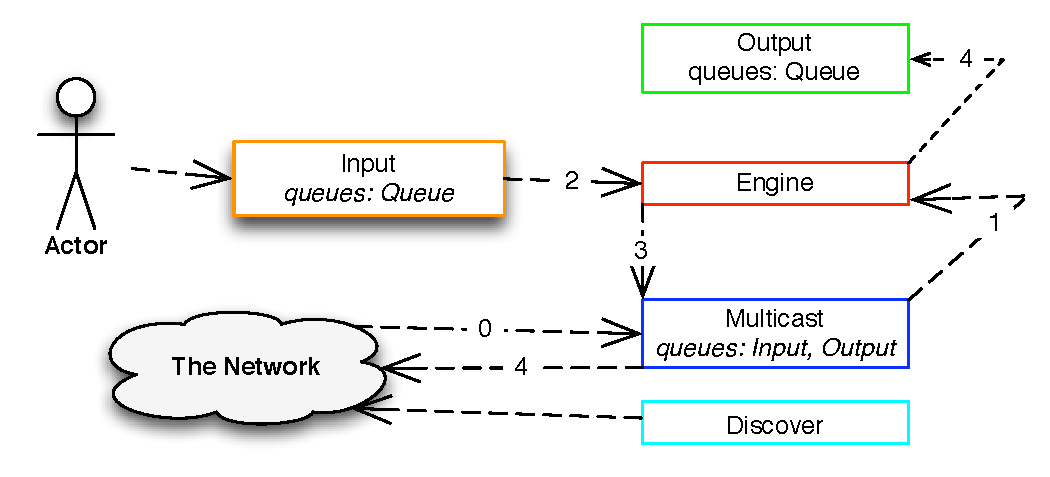
\includegraphics[width=11cm,height=5cm]{diagrams/modules}
      \caption{The 5 modules} \label{fig:modules}
    \end{figure}

    Our game runs in a cycle that is supposed to run many times per second. This means that we assume a certain network and processing speed to be available for playing this game; enough to update every player's screen dozens of times per second and sending and receiving network data. We do not believe that this is unrealistic, given the fact that many games manage to run in this way. We will, however, have to make design decisions which keep the program efficient.

  % subsection design (end)

  \newpage
  \subsection{UML Class diagrams}
  % TODO: Some more explanation.

    \subsubsection{The Input module} % (fold)
    \label{ssub:the_input_module}

      \begin{figure}[!ht]
        \centering
        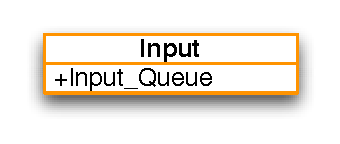
\includegraphics[width=4cm,height=2cm]{diagrams/UML_input}
        \caption{The class diagram for the Input module}
        \label{fig:UML_input}
      \end{figure}

      Figure~\ref{fig:UML_input} shows the input module. The input module handles all keyboard and mouse signals and puts these in the queue ``Input\_Queue''. The engine can access this queue and read all commands given by the player. PyGame will help us with reading user input, but during the writing of this section, we do not know how this should be implemented.
    % subsubsection the_input_module (end)

    \begin{figure}[!ht]
      \centering
      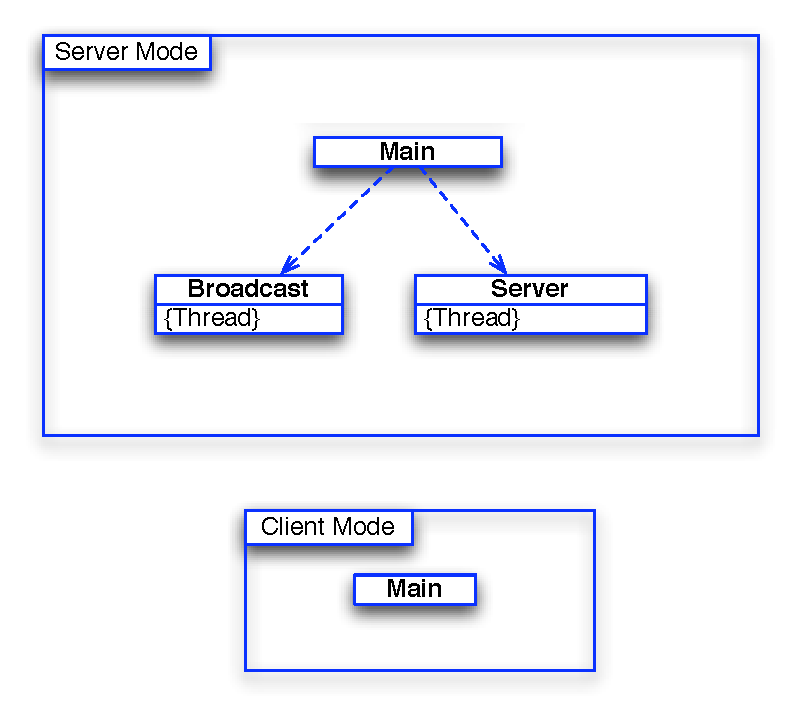
\includegraphics[width=6cm,height=8cm]{diagrams/UML_multicast}
      \caption{The class diagram for the network module} \label{fig:UML_multicast}
    \end{figure}

        \subsubsection{Starting the game and Discovery} % (fold)
        \label{ssub:starting_the_game_and_discovery}
            We use a client/server model for starting a game. One client creates a server, that sends a broadcast message to the entire network. All clients that are waiting to join a game, send a message back to the server. When the server times out, it tells every other client to whom he needs to connect. This makes a token-ring no longer requiring a server.
        % subsubsection starting_the_game_and_discovery (end)

       The blue Network class in Figure~\ref{fig:UML_multicast} is the same class in the network module diagram.

    % subsubsection the_discover_module (end)

    \subsubsection{The Engine module} % (fold)
    \label{ssub:the_engine_module}

      \begin{figure}[!ht]
        \centering
        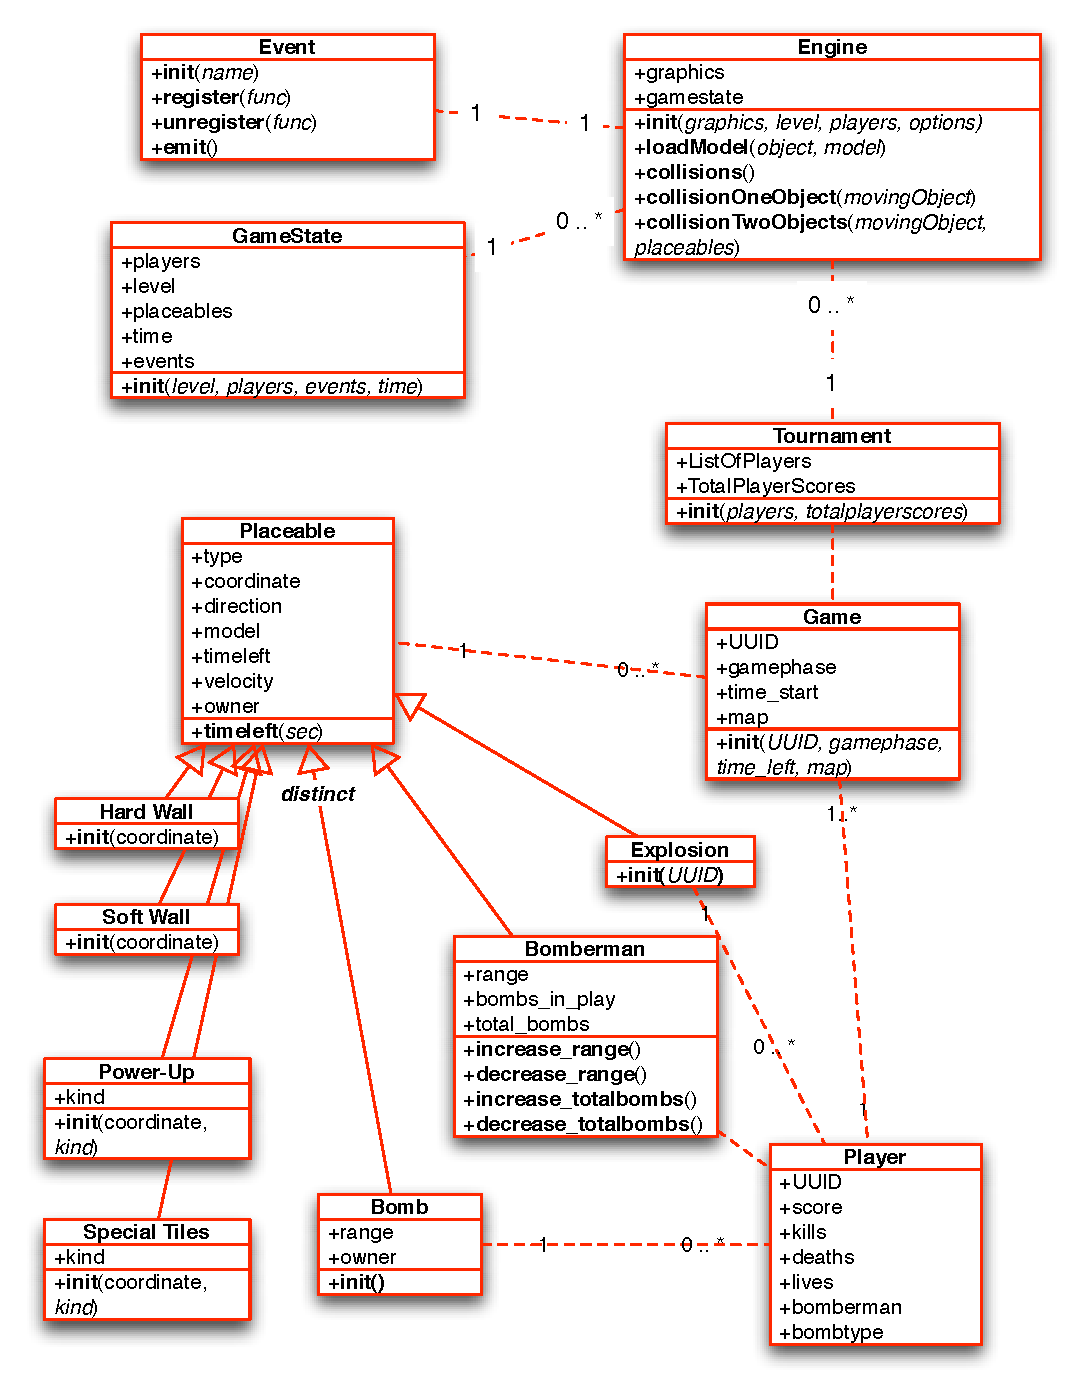
\includegraphics[width=12cm,height=14cm]{diagrams/UML_engine}
        \caption{The class diagram for the game Engine} \label{fig:UML_engine}
      \end{figure}

      \newpage

      A player starts playing the game by creating or joining a \emph{tournament}. A tournament consists of several \emph{games} or rounds that need to be won before an overall winner can be chosen. A game can have one or more players, though, of course, a game with one player in it is not very exciting. For every tournament there is a specific set of rules that states when someone wins or when anyone may join. The tournament class keeps track of all the different players and their total scores over the previous games in the tournament.

      Several games will be played in a tournament consecutively. Only 1 game may be active at any given time, that game will be ``InGame''. The game class handles ending the turn of a player and ending the game, making sure that all data goes to its right spot.

      Every game has its own data, like the time left to play the game. This data is in the \emph{Round} class.

      A \emph{Player} may only be busy with 1 game, he is either waiting to join or he is playing in the active game. This class keeps tracks of the player's score, how many times he has died, where it's standing and what bombs and upgrades belong to it. It also get's the input from both the input module and the multicast module. A player can place a request to move at the controller and to place a bomb.

      The \emph{Level} class keeps track of the size of the board and the lay-out.

      Several objects can be placed in a level. These objects share some properties, brought together in the \emph{Placeable} class. This consists mainly of a location (coordinates) and a texture. A placeable object is one of four types: Hard wall, Soft wall, Explosion or Bomb.\\
        \begin{enumerate}
          \item Hard Wall: this is an object that a player cannot interact with. Placing these wall creates a battle field through wich the player must maneuver, or use to his advantage when placing bombs.
          \item Soft wall: these are wall that can be destroyed by an explosion, but a player pass through it. This gives a player more objects to maneuver through, but can also be used to easily trap a player. When a soft wall is destroyed, it may ``drop'' a \emph{Power-Up} for the player or reveal a special tile.
          \item Bomb: a bomb belongs to a player and blows up when it's timer has reached zero. No player may walk through a bomb, not even it's owner. A player can use this ability to trap another player, but he can also accidentally trap himself.
          \item An explosion: When a bomb explodes, it create cross-shaped explosions, extending horizontally and vertically. These explosions have a place, a short duration of time and an owner. An explosion can set off other bombs, or destroy players, soft walls and power-ups.
        \end{enumerate}

      As has been said before, soft walls which are blown up can leave Power-Ups or reveal a special tile. Power-ups can be, but is not limited to, an increase of range, more bombs, different bombs, and a placeable soft wall \ldots

      A special tile could be a tile that propels a player forward, a tile that changes the direction of an explosion or a tile that transports a player. Special Tiles are not part of basic gameplay and will only be implemented later in the implementation proces.

  Initially, a level consists of coordinates that may have an associated object, like a wall block (indestructible) or a soft-block (destructible) or upgrade (destructible).

      As been said before, soft wall can drop Power-Ups or it can reveal a special tile. A Power-up could be, but not limited to, an increase of the range of your bombs, more bombs to be placed on the field, different bombs, a placeable soft wall \ldots

      A special tile could be a tile that propels a player forward, a tile that changes the direction of an explosion or a tile that transports a player. Special Tiles are not part of basic gameplay and will only be implemented later in the implementation proces.
  
  \textbf{Events}
  
  To connect the engine to the game logic, and to keep that connection flexible and extensible, we are going to use events.
  Events are things that can happen in a game, for example a player dies, a collision occurs, even a player who presses a key.
  
  Events often require something in the gamestate to change. For example when a player dies, he has to be removed from the game and points have to be given to the killing player. And when a player walks against a wall, a collision occurs and that player has to be stopped. So to do that, we'll introduce scripts that handle those things.
  
  A script is a piece of code that is interested in one of more events. So when that event happens, that piece of code gets called and makes changes to the gamestate accordingly.
  
  The big advantage of using events this way is that the engine stays very clean, and the game logic can easily be adjusted. We could easily make a shooter or a tetris game in this engine!
  % subsubsection the_game_module (end)

  \newpage
  \subsubsection{The Output module} % (fold)
  \label{ssub:the_output_module}

  \begin{figure}[!ht]
     \centering
     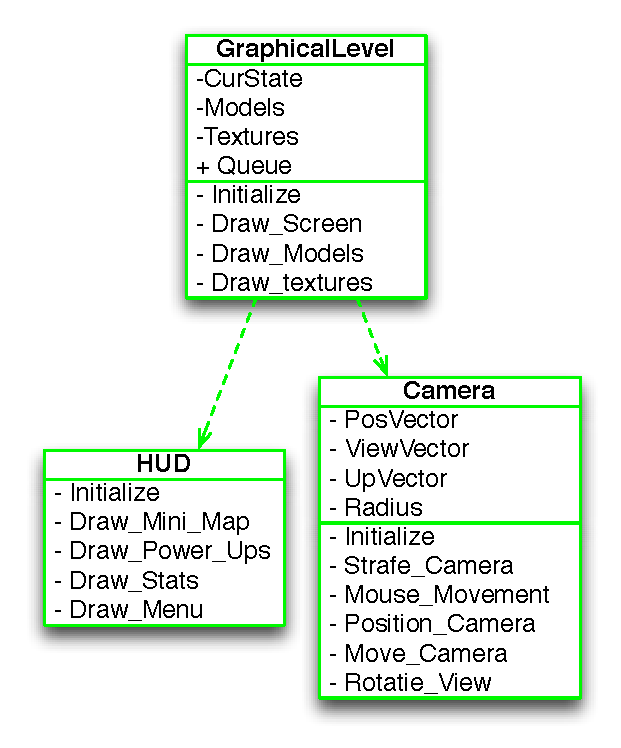
\includegraphics[width=8cm,height=10cm]{diagrams/UML_output}
     \caption{The class diagram for the game's Graphics}
     \label{fig:UML_output}
   \end{figure}

   \textbf{Screen} \\
   The Output module gets a game state as input from the game engine and updates the screen. This screen consists of a 3D level and 2D layer on top of the 3D level. The 3D level is drawn according to the view of the camera and consists of a 3D world with all kinds of objects. The 2D layer consists of a minimap, the player's stats, and the player's power ups, which are all drawn. The Graphics module consists of three classes, namely: the GraphicalLevel class, the HUD class, and the Camera class.
   
   The GraphicalLevel class is the 3D level. It keeps the current game state, the models that are to be drawn and the textures that are used. After it is initialized, it can draw the 3D scene, draw the models, and apply the textures. The main use of this class is updating the 3D level based on the game state delivered by the game engine. It makes use of the two other classes to fully update the screen.
   
   The HUD class is a 2D layer on top of the 3D level. It draws the mini map, the power ups, the stats, and possible an in-game menu when activated. This class is used to update the 2D HUD layer on top of the 3D level based on the game state delivered by the game engine.
   
   The Camera class handles the camera movement. It can move the camera forward and backward, left and right, and rotate the camera, according to the user input delivered by the game engine. It is used as first-person view in the 3D level.
   
   \textbf{Sound} \\
   The Output module will also handle sounds when we have time left to implement it. There are some basic sounds stored, like explosions, walking etc. which will be played at certain in-game events. This means that certain keys and events will toggle a certain sound. For example when a player gets killed or kills, when a player has won, pressing an ``Activate powerup'' key etc.
   
   All the sounds will be implemented in the GraphicalLevel class, since the sounds ``change'' the 3D level. The sounds don't change the 3D level physically, but they do change the experience in the 3D level.
     % subsubsection the_output_module (end)

% section program_modules (end)
